\documentclass[10pt]{article}
\usepackage{latexsym}
\usepackage{natbib}
\usepackage{graphicx}
\usepackage{subfigure}
\usepackage{listings}
\usepackage{algorithm}
\usepackage{algpseudocode}
\usepackage{amsmath}
\usepackage{amssymb} 
\usepackage{amsthm}

\newtheorem{definition}{Definition}
\newtheorem{theorem}{Theorem}

\newcommand{\R}{\mathbb{R}}
\newcommand{\E}{\mathrm{E}}
\newcommand{\Cov}{\mathrm{Cov}}
\newcommand{\Var}{\mathrm{Var}}

\title{MCMT Project Report\\Mixing Time in Reinforcement Learning}
\author{Shun Zhang}
\date{}

\begin{document}
\maketitle

\section{Introduction}

Reinforcement Learning is a learning method for the problem of learning with
feedback from the environment. In the literature of Reinforcement Learning,
Markov Decision Process is generally used to model the environment. There are
many learning algorithms defined on the Markov Decision Process. However, even
though most of the algorithms are proved to eventually converge to the optimal
solution, the time required to achieve a near-optimal solution is not
theoretically bounded.  In this report, I use mixing time to analyze the
convergence time.

%This report is organized as follows. Section~\ref{sec:mdp} gives standard
%definitions for Markov Decision Process. 

\section{Markov Decision Process}
\label{sec:mdp}

Markov Decision Process (MDP) can be regarded as an extension to Markov chain.
If an agent starts in a state in a Markov chain, it can only drift according to
the transition probability. It cannot indicate its preference on where to go. In
MDP, the states have rewards defined on them. The agent obtains the reward when
reaching a state. It wants to maximize the rewards it gets over time, so we
introduce {\em actions} in MDP.

MDP is defined below compared to the definition of Markov Chain using the same
notations.

\begin{definition}
Markov Chain is a two-element tuple $(\Omega, P)$, where
\begin{itemize}
\item $\Omega$ is the state space.
\item $P$ is the transition probability. $P: \Omega \times \Omega \rightarrow
\R$.
\end{itemize}
\end{definition}

\begin{definition}
Markov Decision Process is a four-element tuple $(\Omega, A, P, R)$, where
\begin{itemize}
\item $\Omega$ is the state space.
\item $A$ is an action set.
\item $P$ is the transition probability. $P: \Omega \times A \times \Omega
\rightarrow \R$.
\item $R$ is the reward upon reaching a state. $R: \Omega \rightarrow \R$.
\cite{rl}
\end{itemize}
\end{definition}

There is a difference in the transition probability compared to Markov chain ---
it measures the probability reaching another state, given a state and an action.

We use the term utility to describe the accumulated rewards after starting from
a state.

\begin{definition}
A policy in a MDP is a mapping $\pi: \Omega \rightarrow A$.
\end{definition}

\begin{definition}
The utility of a state $s$ following policy $\pi$ is: $U(s) = \E (R(s) + \gamma
R(s_1) + \gamma^2 R(s_2) + \cdots)$, where $\gamma \in (0, 1]$, is a discounting
factor.
\end{definition}

\section{Learning Algorithms}
\label{sec:dm}

The learning process is represented by updating {\em utility}, which evaluates
the expected accumulated payoff starting from a state. 

The goal of the agent is to maximize the accumulated rewards it gets. Usually, the agent should take the action that leads to the maximum expected
utilities, that is ${\mathrm{argmax}}_a \sum_{s'} P(s, a, s') (R(s') + \gamma
\hat{U}(s'))$.  However, the
$U$ may be inaccurate, it may also want to explore the actions randomly with
some probability. The is called the Explore or Exploit Dilemma --- exploration
may takes the agent to the subset of the states with higher rewards that are
previously not realized. One popular way to resolve this dilemma. is called $\epsilon$-greedy, which the agent
takes the action that maximizes the estimated utility with probability $1 -
\epsilon$, and takes a random action with probability $\epsilon$.

We introduce two learning algorithms. One is model-based, which assumes that we
know $R$ and $P$. The other is model-free, which assume that we don't know $R$
or $P$.

\subsection{Value Iteration}

\begin{theorem}
The utility for the optimal policy satisfies $U(s) = \max_a \sum_{s'} P(s, a,
s') (R(s') + \gamma U(s'))$ for all $s$.
\cite{rl}
\end{theorem}

To update, we can use the following rule. This is a bootstrapping way to solve
the nonlinear equations above.

\begin{equation}\label{eq:vl}
U(s) \leftarrow \max_a \sum_{s'} P(s, a, s') (R(s') + \gamma U(s'))
\end{equation} 
This assumes that we know the transition and the reward functions.

\subsection{Q-learning}

When the transition and reward functions are not known, computing $U$ won't be
helpful for decision making. We define a new function that evaluates a state,
action pair.

\begin{definition}
$Q(s, a) = \sum_{s'} P(s, a, s') (R(s') + \gamma U(s'))$.
\end{definition}
Note that by definition, $U(s) = \max_a Q(s, a)$. The $Q$ function can be
computed by the following update rule.

\begin{equation}\label{eq:td}
Q(s, a) \leftarrow (1 - \alpha) Q(s, a) + \alpha (R(s') + \gamma \max_{a'} Q(s',
a'))
\end{equation} 
where $\alpha \in (0, 1)$. 

\begin{theorem}
Following the update rule Equation~\ref{eq:td}, $Q$ eventually converges to $Q^*$.
\cite{rl}
\end{theorem}

Note that Q-learning doesn't give any bound on convergence. Actually, this is
affected by the transition model.

\section{Convergence Rates of Utilities}

One measure of the learning performance is to compare the current utility with
that of the optimal solution, that is $\sum_s ||U(s) - U^*(s)||$ or $\sum_{s,a}
||Q(s, a) - Q^*(s, a)||$ for $s \in \Omega$.

\begin{figure}[h!]
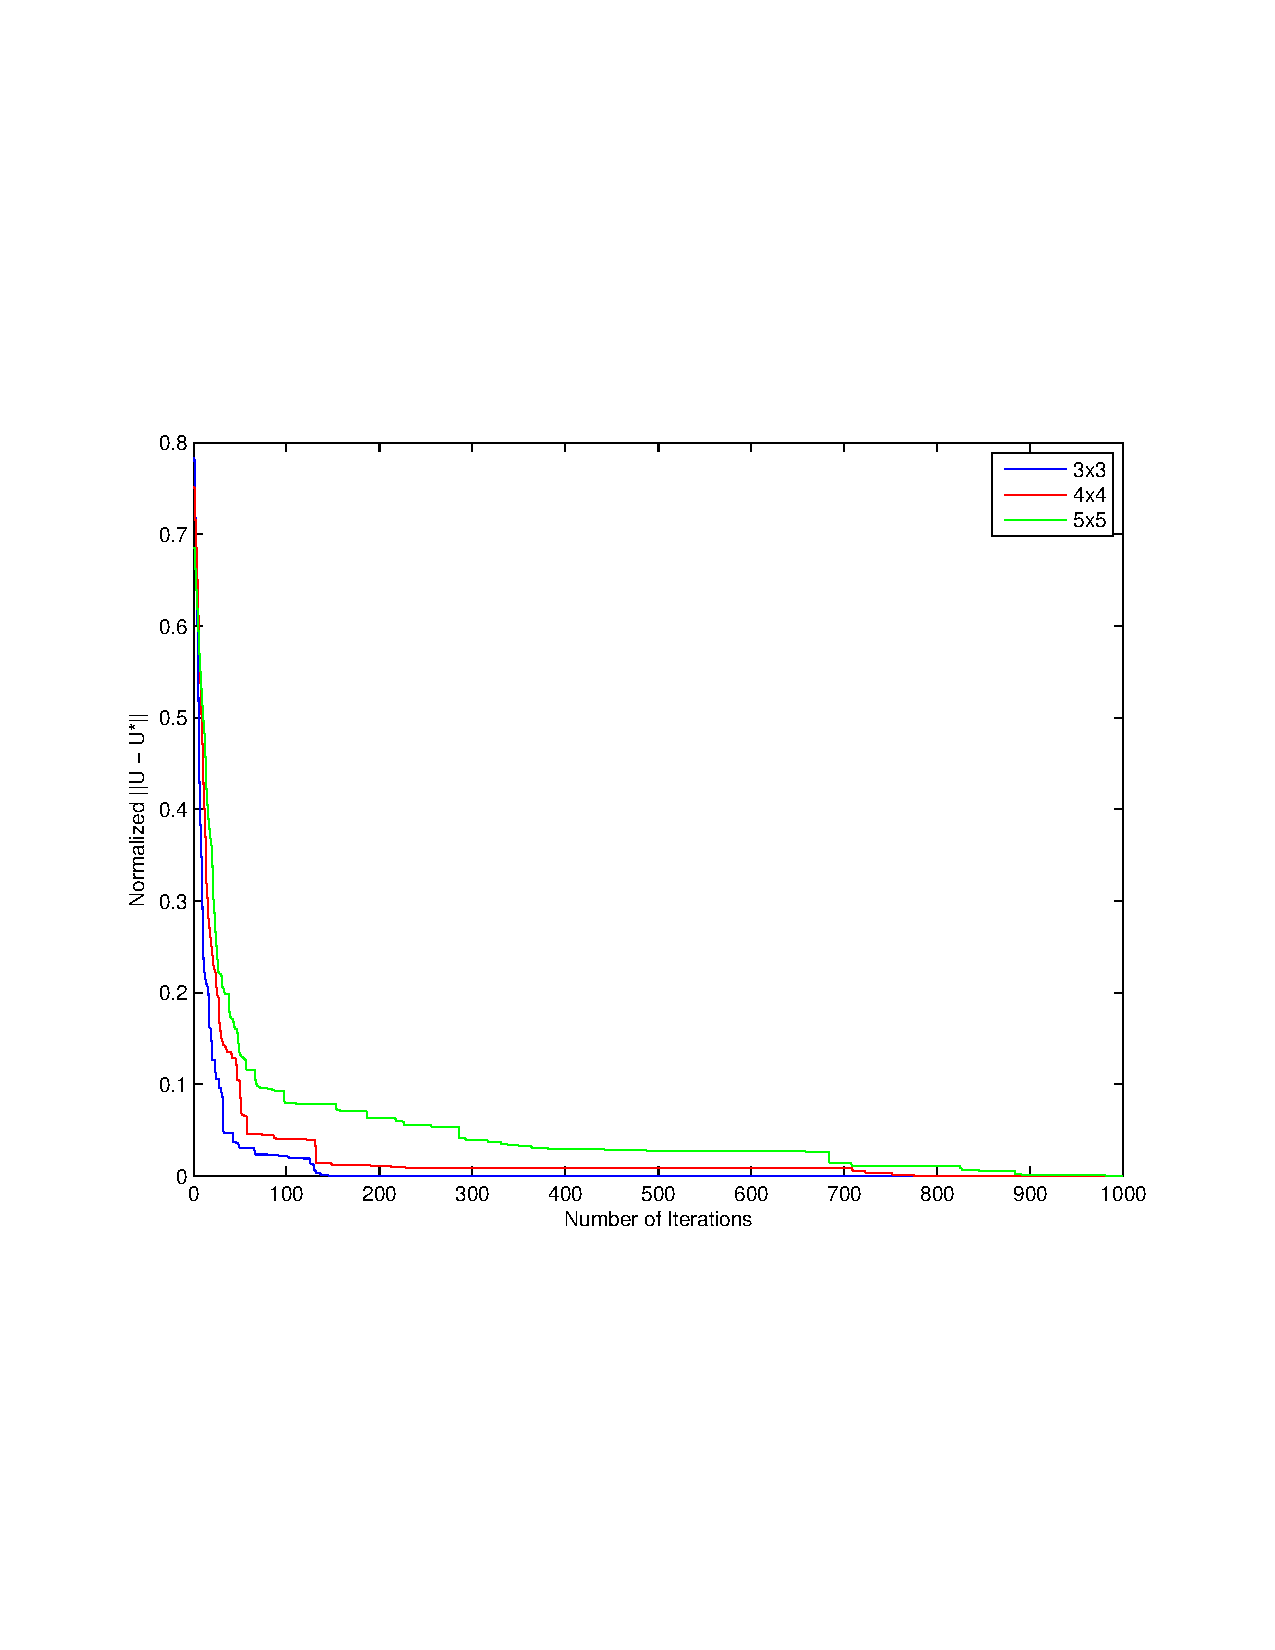
\includegraphics[width=0.5\textwidth]{exp0.pdf}
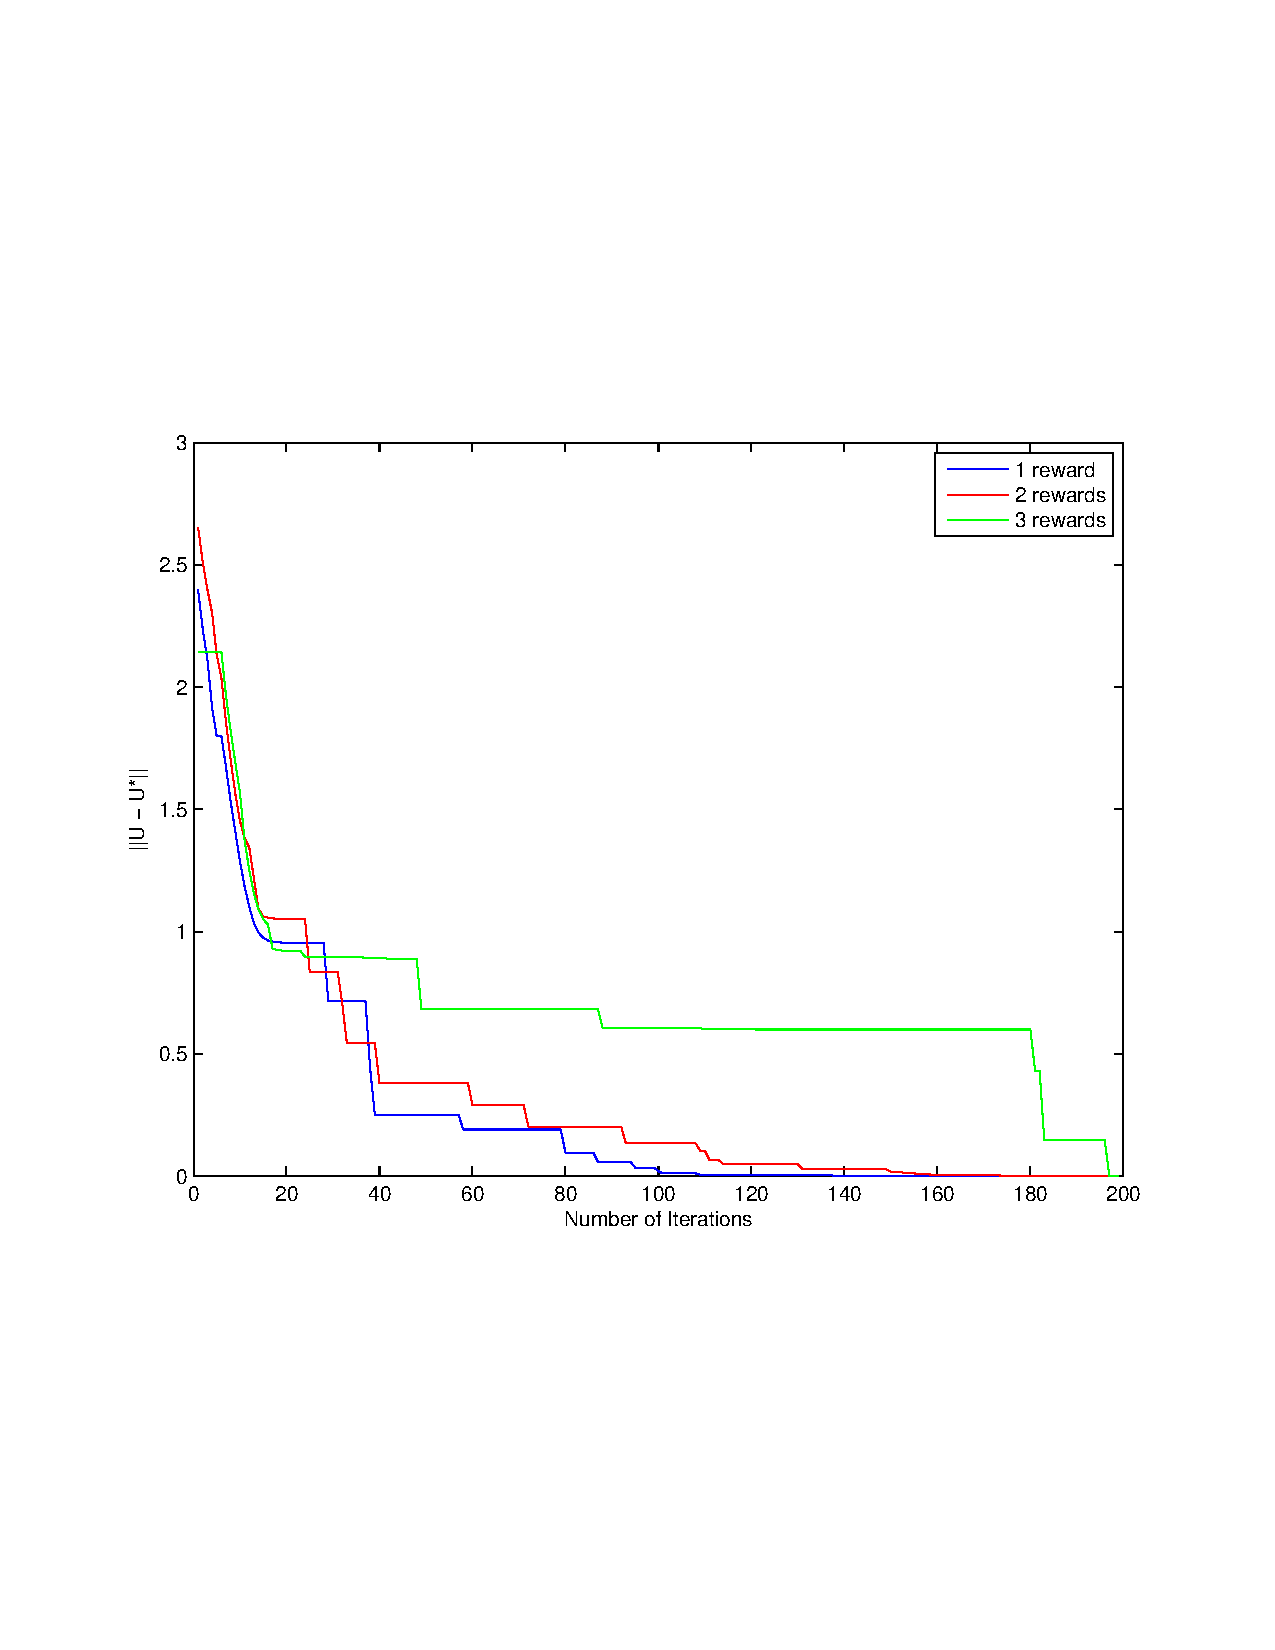
\includegraphics[width=0.5\textwidth]{experiment.pdf}
\caption{(Left) Convergence rates of different domains, with sizes of 3x3,
4x4, 5x5. (Right) Convergence rates of domains with size 4x3 of different number
of rewards.}
\label{fig:exp}
\end{figure}

I evaluated the Q-learning algorithm in gridworld domains, with the sizes of
3x3, 4x4 and 5x5. Apparently, the mixing time of the transition models for these
domains vary. The convergence rates of $U$ differ. This is shown in the left
figure in Figure~\ref{fig:exp}.

In the second experiments, I evaluated Q-learning in 4x3 gridworld domains but
with different number of rewards, 1, 2, 3, respectively. The result is shown in
right figure in Figure~\ref{fig:exp}. In the figure, the $U$ converges to its
optimum slowly when there are more rewards to consider, even though the
transition functions are same for all these three settings.

\section{Mixing Time in Literature}

Kearns et al. proposed the idea of using mixing time on utility as a metric for
learning performance \cite{kearns2002near}. Their main contribution of
the paper is an innovative algorithm that takes mixing time of the transition
function into consideration. Their new algorithm, Explicit Explore or Exploit
(E$^3$), shows that the mixing time of the learning algorithm can be
polynomially bounded by the mixing time of the transition function. The idea is
that the agent needs to visit a state a certain number of times to mark it as
{\em known}. The mixing time of the transition matrix is an important factor for
such confidence.

This encourages the agent to cover the state space efficiently, and expedite
the convergence of $U$. Even though, this doesn't outperform traditional
algorithms in other metrics, for example, minimizing the regrets. Regrets are
defined as the difference between the rewards got in the simulation and the
rewards the agent could have got. In Q-learning, for example, the agent may
stick to any reward it observes while exploring. In E$^3$, the agent explicitly
drops the chance to collect small rewards, but tries to explore the state space.

The main theorem of their work is as follows.

\begin{theorem}
\label{thm:e3}
Let $U^∗(i)$ denote the value function for the policy with the optimal expected
discounted return in M. Then there exists an algorithm A, taking inputs
$\epsilon,\delta,N$ and $U^∗(i)$,such  that  the  total  number  of  actions  and  computation
time  taken  by  $A$ is  polynomial  in $1/\epsilon,1/\sigma,N$,the mixing time
of the transition function \footnote{It is horizon time in the original paper
for the discounted case. They use the term mixing time for the undiscounted
case, that is, when $\gamma = 1$.}, and the maximum reward. With probability at
least $1-\delta$, $A$  will halt in a state $i$, and output a policy such that
following such policy, $U(i) \geq U^*(i) - \epsilon$.
\end{theorem}

In Theorem~\ref{thm:e3}, the authors claim that the utility of the states can be
polynomially bounded by some factors of the domain, including the mixing time of
the optimal policy.
Another related work is a more popular algorithm R-max \cite{rmax}, following
Kearns et al., that makes the distinction of exploration and exploitation phases
implicit.

\section{Discussion and Conclusion}

In this project, I introduced the concept of reinforcement learning, and how it
is related to Markov Chain. I generated empirical data of the convergence time
of utilities of a grid world domain. An application of mixing time is also
surveyed in the literature.

\begin{figure}[h!]
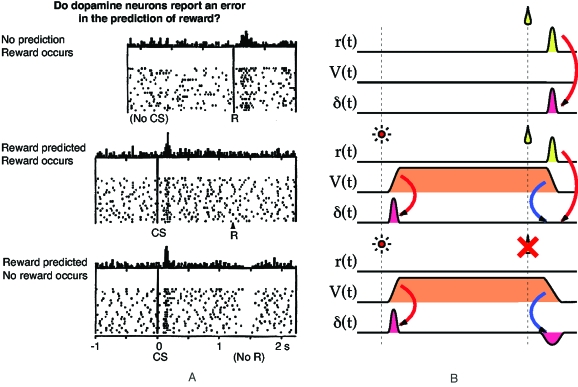
\includegraphics[width=0.9\textwidth]{dopamine.jpg}
\label{fig:nat}
\end{figure}

To conclude, there is a journal article in neuroscience that shows a correlation
between the dopemine that a creature fires and the temporal difference error
\cite{tanaka2004prediction}.  The temporal difference error is defined as $R(s')
- (\gamma U(s') - U(s))$. This means that, if the agent uses $U$ to make
decisions, how unexpected he feels after a step. The temporal difference error
can occur when an unseen reward time is observed for the first time, or a reward
that is believed to exist is missing. One experiment of this paper is shown in
Figure~\ref{fig:nat}. In the top subfigure, the temporal difference error is
positive when a monkey observes a banana. In the bottom figure, the temporal
difference error is negative when the banana is missing, while it is supposed to
be there. So it is possible that animals use a reinforcement-learning-like
approach to learn the world.

\bibliographystyle{plain}

\bibliography{report}

\end{document}
